\documentclass{article}
\usepackage[margin=1.2in]{geometry}
\usepackage{datetime}
%\usepackage{hyperref}      %for \url macro
\usepackage{microtype}     %attempt to fix issue with justification protrusion (in references)
\usepackage{amssymb}       % for formatting less/greater than symbols
\usepackage{amsmath}
\usepackage{enumitem}      %for changing spacing in bulleted lists
\usepackage{subfigure}        %for subfigures


\renewcommand{\arraystretch}{1.25}

\usepackage[gobble=auto, runall=true]{pythontex}
\usepackage{float} %for forcing position of images

\usepackage{graphicx}
\graphicspath{ {../images/} }
\usepackage[export]{adjustbox}
\usepackage[justification=centering]{caption}

\usepackage{listings}   %for typesetting code
\usepackage{color}
\definecolor{codegreen}{rgb}{0,0.6,0}
\definecolor{codegray}{rgb}{0.5,0.5,0.5}
\definecolor{codepurple}{rgb}{0.58,0,0.82}
\definecolor{backcolour}{rgb}{0.95,0.95,0.92}
\lstdefinestyle{mystyle}{
    backgroundcolor=\color{backcolour},
    commentstyle=\color{codegreen},
    keywordstyle=\color{codepurple},
    numberstyle=\tiny\color{codegray},
    stringstyle=\color{codepurple},
    basicstyle=\footnotesize,
    breakatwhitespace=false,
    breaklines=true,
    captionpos=b,
    keepspaces=true,
    %numbers=left,
    numbersep=5pt,
    showspaces=false,
    showstringspaces=false,
    showtabs=false,
    tabsize=2
}
\lstset{style=mystyle}

\frenchspacing                   %removes extra spacing after a period at the end of a sentence.
\newdateformat{daymonthyear}{\THEDAY\ \monthname\ \THEYEAR}

\title{CSC411 Machine Learning \\ Project 2: Deep Neural Networks}
\author{ Ariel Kelman \\ Student No: 1000561368
         \\ \\
         Gideon Blinick \\ Student No: 999763000 }
\daymonthyear



\begin{document}
   \maketitle{}


   \section{Introduction}
   This section provides an introduction to Project 2, including the data used, and notes
   on reproducing the results. Sections 2-6 discuss the implementation of a simple neural
   network to classify images from the MNIST database, section 7 is a theoretical anlaysis
   of the efficiency of backpropogation, and sections 8-10 work with deep neural networks.

   \subsection{Digits}
   The following figure shows 10 random images from the training set of each of the digits.
   \begin{figure}[H] \centering
      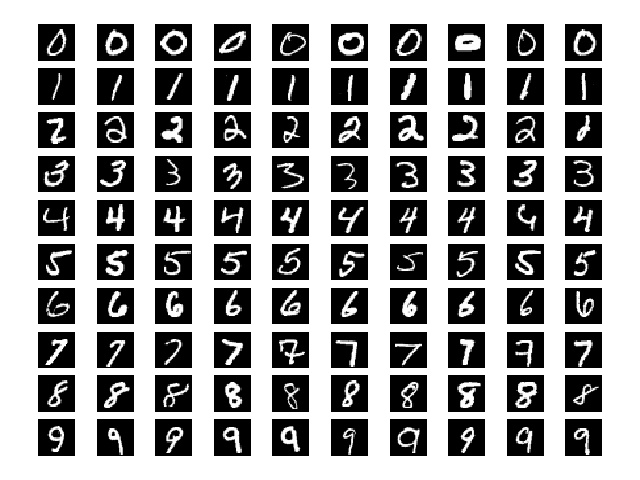
\includegraphics[width=4in]{resources/part1}
      \caption{10 random samples from the training set for each digit. This image
         was generated using \texttt{plot\_samples()}. }
   \end{figure}
   The data was downloaded from the assignment webpage, and imported into Python using the
   provided code. The data was already divided into training and testing sets.

   \subsection{Results \& Report Reproducibility}
   All results and plots can be generated using the appropriate python files.
   Code for sections 1-6 can be found in \texttt{digits.py}, for part 8 and 9 in \texttt{faces.py},
   and for part 10...
   Running the code will save all generated images in the \texttt{resources} folder,
   where they are used by \LaTeX. Note that some of the sections require the code for
   other sections to be run first.
   To reproduce the report, simply run it through \LaTeX.


   \section{The Network}
   The following function implements a neural network with no hidden layers, with the
   output passed through a softmax layer to estimated probabilities.

   \begin{lstlisting}[language=Python]

      def no_hidden_layers(x, W, b):
   	    '''Compute the network'''
      	 #the first column of W contains the weights for output 1
       	 # W is (784x10), x is (784x60 000) and b is (10x60 000)
       	 # So L1 is (10x60000)
      	 L1 = np.dot(W.T, x) + tile(b, (1, np.shape(x)[1] ) )
     	 return softmax(L1)
   \end{lstlisting}

   The network is described by the weights and biases from the 784 = 28*28 inputs
   (representing pixel intenisites of the input image) to ten ``output'' nodes
   (with the identity as the activation function). The output from this layer is what is
   passed through the sofmax function $p_k = \frac{ e^{o_k} }{ \sum_q e^{o_q}}$.

   The weights are represented as a 784 by 10 matrix $W$, where $w_{ij}$ ($i^{th}$ row, $j^{th}$
   column) represents the weight from the $i^{th}$ input to the $j^{th}$ output.
   When computing the network on a given sample, the transpose of $W$ is multiplied
   by the column vector (or matrix when computing on multiple samples) representing the input.
   The biases are represented by a 10 by 1 vector, one entry for each output. We use the \texttt{tile()} function
   to duplicate the biasses $b$ up to appropirate dimensions (10 by 60000) to be added to the result of $W^T X$.

   Throughout the code, $y\_$ is a matrix representing the correct results for each image; each column is a
   vector of zeros with a 1 in the place representing the correct digit.
   $y$ is a matrix representing the output probabilities from the network of the same dimensions
   as $y\_$ (in the derivations below, as well as some comments on the code, $p$ is used in place of $y$);
   each column is a vector representing the probabilities for each digit for a particular sample.

   \section{Gradient}
   The cost function is taken to be $- \sum_{k} y_k ln(p_k)$ for one sample, where $y_k$ is
   1 for the correct class and 0 otherwise, and $p_k$ is the prediction probability for class k.
   Writing this in vector notation (replacing the sum with a vector dot product) and
   summing over all the samples gives:
      \begin{equation*} \begin{split}
         C = - \sum_{s} y^{(s)} ln(p^{(s)})
      \end{split} \end{equation*}
   where $ln$ is applied pointwise, and $s$ is an index over the samples. $y^{(s)}$ is
   a vector of 0's with a 1 in the position representing the correct digit.

   The following results will be used in the derivations throughout this section:
      \begin{equation*} \begin{split}
        \frac{ \partial p_k}{ \partial o_q } =
            \begin{cases}
               -p_k p_q       & \textrm{ if } k \neq q \\
               p_q (1 - p_q)  & \textrm{ if } k = q
            \end{cases}
      \end{split} \end{equation*}
   These results follow directly from the definition of the softmax function.


   \subsection{Gradient wrt $w_{ij}$}
   First, we derive $\frac{ \partial C}{ \partial o_q }$ (for one sample), to be used in the derivation of
   $\frac{ \partial C}{ \partial w_{ij} }$.
      \begin{equation*} \begin{split}
        \frac{ \partial C}{ \partial o_q }
           &= \bigg[   \frac{ \partial C}{ \partial p_q } \frac{ \partial p_q}{ \partial o_q }    +   \sum_{k \neq q} \frac{ \partial C}{ \partial p_k } \frac{ \partial p_k}{ \partial o_q }  \bigg]  \\
           &= - \bigg[    y_q \frac{1}{p_q} p_q (1 - p_q)  +   \sum_{k \neq q} y_k \frac{-1}{p_k} p_k p_q  \bigg]  \\
           &= - \bigg[    y_q (1 - p_q)  -  \sum_{k \neq q} y_k p_q       \bigg]   \\
           &=   \bigg[    - y_q  +  \sum_k y_k p_q   \bigg]  \\
           &=  p_q - y_q
      \end{split} \end{equation*}
   The last line follows because $\sum_k y_k = 1$. Using this result, and applying the chain rule
   gives:
      \begin{equation*} \begin{split}
        \frac{ \partial C}{ \partial w_{ij} }
           &= \frac{ \partial }{ \partial w_{ij} } \sum_{s} y^{(s)} ln(p^{(s)}) \\
           &= \sum_s \sum_q  \frac{ \partial C}{ \partial o_q } \frac{ \partial o_q }{ \partial w_{ij} } \\
           &= \sum_s \sum_q ( p_q - y_q ) x_i \delta_{jq}  \\
           &= \sum_s ( p_j - y_j ) x_i
      \end{split} \end{equation*}
   As the outputs are linear functions of both the inputs and the weights, the derivative
   with respect to a weight is given by the value of the input to that weight, namely $x_i$.
   The Kronecker delta $\delta_{jq}$ results from $ \frac{ \partial o_q }{ \partial w_{ij} } $
   being nonzero only when $j = q$.
   The $(s)$ superscript indicating the sample index was omitted throughout the derivation for clarity of presentation.

   \subsection{Vectorized Gradient Code}
   The following code computes the gradient with respect to the wieghts and biases
   (representing all input training images in a matrix $X$, 784 by the number of samples, in this case 60000):
      \begin{lstlisting}[language=Python]

         def grad(y_, y, x):
      	   '''Compute the gradient wrt weights and biases'''
          	#y and y_ have dimension (10x60000)
          	#x has dimension (784x60000)

          	diff = (y - y_) #y is output of softmax
              	# diff is p_j - y_j

          	grad_W = np.dot( x, diff.T )
          	grad_b = np.sum( diff, 1)
          	grad_b = np.reshape(10,1)

          return  grad_W, grad_b
      \end{lstlisting}

   The above code works by creating a matrix $\nabla C $ which is of dimension 784x10
   (same as the weight matrix), and where every element contains $\frac{ \partial C}{ \partial w_{ij} }$ for the corresponding $w_{ij}$.
   It does this by implementing $\sum_s ( p_j - y_j ) x_i$ for each matrix element, where $i$ increases as you go down
   a column (from 1 to 784) and $j$ increases as you go accross a row (from 1 to 10). Each element itself contains 60000
   terms added together to aggregate the information from all samples.

   \section{Training}
   The neural network was trained on the full training set of $60000$ images without momentum.
   The weights and biases were initialized using a uniform distribution to values between $0$ and $1$.
   A learning rate of $10^{-4}$ was used for $1000$ iterations, giving a training accuracy of $92.6\%$,
   validation accuracy of XXX, and a testing accuracy of $92.2\%$.
   To determine the optimal learning rate, the function \texttt{optimize\_rate()} tested several
   learning rates, outputting the validation accuracy for each. Learning curves for each weight
   are saved as images in the \texttt{resources} directory.

   The following figure shows the learning curve for the final parameters used:
     \begin{figure}[H] \centering
         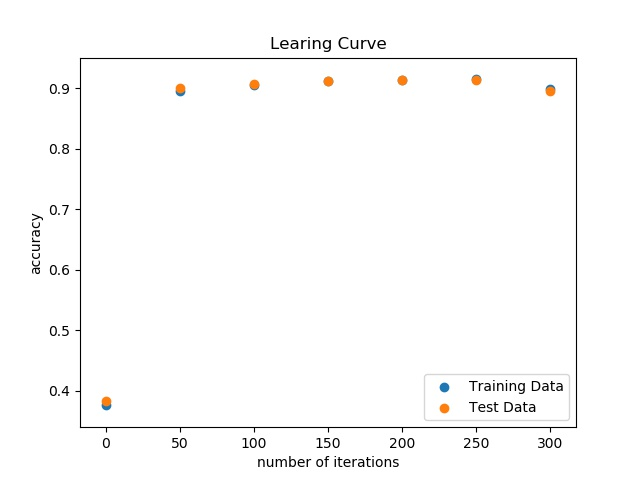
\includegraphics[width=4in]{resources/part4}
         \caption{Learning curve with a learning rate of $10^{-4}$. }
      \end{figure}

  The following figure, generated using \texttt{image\_W()} shows the weights input to each
  output neuron (before the softmax layer), corresponding to the digits $1...10$:
     \begin{figure}[H] \centering
         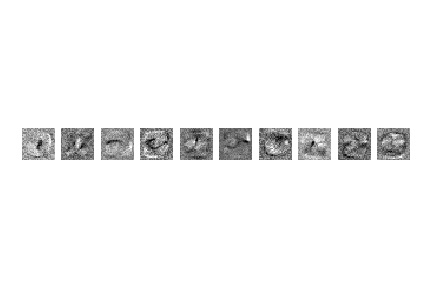
\includegraphics[width=4in]{resources/weights}
         \caption{Visualization of the weights }
      \end{figure}





   \section{Training with Momentum}
   The neural network was trained on the full training set of $60000$ images with momentum, set to $xxx$.
   A learning rate of $xxx$ was used for $xxx$ iterations, giving a training accuracy of $xxx$
   and a testing accuracy of $xxx$.
   The weights and biases were initialized using a uniform distribution to values between $0$ and $1$.

   The following figure shows a learning curve...


   \section{Analysis of Momentum}
   For the analysis in this section, the weights $w_{ab}$ and $w_{cd}$ were used (recall that $W$ is
   a $784$ by $10$ matrix). After training the network as described in the previous section,
   these weights had the values $w_{ab} = xxx$ and $w_{cd} = yyy$.

   \subsection{Contour Plot}
   The following plot shows the variation of the cost function (negative log loss) around the
   values for $w_{ab}$ and $w_{cd}$ chosen above.

   \subsection{Trajetory without Momentum}

   \subsection{Trajetory with Momentum}

   \subsection{Discussion}




   \section{Efficiency of Vectorized Backpropogation}
   Consider a fully connected neural network with $N$ layers each containing $K$ neurons. By convention,
   the input layer will not be counted toward $N$ layers, but the final output layer will be
   counted (thus there are $N$ sets of weights and biases that must be learned). Any function
   (such as softmax) applied to the final layer is ignored; none of these conventions will
   affect the asymptotic runtime. We also assume that the results of the forward pass of the
   network are cached, to be used for both vectorized backpropogation and computing the
   gradient with respect to each weight independenly.
   We can also ignore the biases; including them could be accomodated by adding an extra
   neuron to every layer (except the last) with a constant value of $1$. This would be
   equivalent to increasing $K$ by $1$. As a final note, any functions (such as softmax) applied
   to the output are ignored; these would have no asymptotic effect on $N$ and would increase
   linearly with $K$.

   Denote each layer by the numbers $1,2... N$ (we can refer to the input layer as layer $0$).
   The efficiency of computing the gradient with respect to a weight to/from a particular layer
   does not depend on which weight it is, so $w^{a}$ can stand for an arbitrary weight from
   layer $a-1$ to $a$. A particular neuron in layer $n$ will be denoted by $\sigma^n$ with a
   subscript to denote that one specific neuron in the layer is intended (the one which the
   weight under consideration leads to).

   Then the following holds: %h, m, q
      \begin{equation*} \begin{split}
        \frac{ \partial C}{ \partial w^{N} }
           &= \frac{ \partial C}{ \partial \sigma^N_q }  \frac{ \partial \sigma^N_q}{ \partial w^{N} } \\
        \frac{ \partial C}{ \partial w^{N-1} }
           &= \sum_q^K \frac{ \partial C}{ \partial \sigma^{N}_q }  \frac{ \partial \sigma^{N}_q }{\partial \sigma^{N-1}_m}  \frac{ \partial \sigma^{N-1}_m }{ \partial w^{N-1} } \\
        \frac{ \partial C}{ \partial w^{N-2} }
           &= \sum_q^K \sum_m^K \frac{ \partial C}{ \partial \sigma^{N}_q }  \frac{ \partial \sigma^{N}_q }{\partial \sigma^{N-1}_m}   \frac{ \partial \sigma^{N-1}_m }{\partial \sigma^{N-2}_h}   \frac{ \partial \sigma^{N-2}_h }{ \partial w^{N-2} } \\
      \end{split} \end{equation*}
   Again, in each case, the derivative of the last neuron ($\sigma_q, \sigma_m, \sigma_h$ respectively in the
   equalities above) with respect to a weight leading to that layer refers to the neuron where
   that weight terminates.
   Since there are $K$ neurons in each layer, each sum goes up to $K$.

   With $K$ neurons in each layer, there are $K^2$ weights between layers; thus the efficiency of
   finding $ \frac{ \partial C}{ \partial w^{N} } $ for a specific weight is $O(1)$ with respect
   to $N$ and $K$, but for all the weights is $O(K^2)$.
   For a specific weight into layer $N-1$, the efficiency would be $O(K)$; scaling this to
   all the weights is $O(K^3)$, since the results for other weights are not cached.
   Continuing this trend backward (each sum adds a factor of $K$), the efficiency of finding the derivative of all the weights
   into the second hidden layer is $O(K^{N})$.
   If we make the simplifying assumption that there are $K$ input neurons, then the efficiency
   of finding all the derivatives for the weights in the first layer is $O(K^{N+1})$.
   Taking only the highest order, gives an overall efficiency of $O(K^{N})$.

   The exponential dependence on $N$ also follows intuitively - as adding and extra layer
   exponentially increases the number of paths from the cost to the weight, and to find
   the derivative, each of these paths must be followed.

   For vectorized backpropogation, the derivative of the cost with respect to each layer
   can be computed using the cached values and matrix multiplication. Ignoring the complexity
   of carrying the derivative through the activation function, the derivative with respect to
   each weight between layers $N-1$ and $N$ requires just one matrix multiplication.
   Moving backward through each layer adds one more matrix multiplication.
   With each layer having $K$ neurons, these matrices have dimension $K$ by $K$.
   The complexity of matrix multiplicaion is polynomial in their dimensions; multiplying two
   $K$ by $K$ matrices has complexity $O(K^3)$ (there are algorithms with slightly lower powers,
   but we'll take $3$ as a baseline here). Therefore, to compute the gradient with respect to all
   the weights from the input to the first hidden layer is $O(N K^3)$, and if this is done
   one matrix at a time (i.e. propogating backwards one layer at a time), the derivative
   with respect to all the intermediate weights falls out at no extra cost (they are the
   result of already computed matrix multiplications).
   Thus the complexity of vectorized backpropogation with caching is $O(N K^3)$ for a
   network with $N$ layers (excluding the input layer) each of $K$ neurons.

   For large neural networks, particularly those with several hidden layers, fully vectorized
   and cached backpropogation reduces the asympotic runtime from to exponential in $N$ to being
   linear in $N$, a huge speedup.


   \section{Classifying Faces}
   The data for this section was downloaded using the file \texttt{get\_data.py}. Carrying over
   a blacklist for bad images from Project 1, and adding in a check to ensure the hashes were
   correct, the images were downloaded, converted to grayscale, and cropped according to the given
   bounding box. The resulting image was rescaled to $32$ by $32$ pixels.
   While over 90 images were downloaded for Lorraine Bracco, Angie Harmon, Alec Baldwin,
   Bill Hader, and Steve Carell, only 57 images were downloaded for Peri Gilpin.
   Therefore, 70 images were used in the training set for each actor, while 37 were used for Gilpin,
   leaving 20 images (per actor) for the validation and test sets. Rather than use an
   additional 10 images for the test set (for 20 test images per actor), and possibly even doing
   the same for the validation set, cross-validation (i.e. choosing the training/validation/testing
   set differently) was used as described below.

   The supplied code was modified to create a fully connected, single hidden layer (with RELU
   activation function) neural network. The data was loaded and formatted using the \texttt{format\_data()}
   function, which creates a dictionary similar to the format in which the MNIST data was loaded:
   a key for the training, validation, and testing set for each actor, with the value holding a
   \texttt{numpy} array holding the appropriate data.
   The function \texttt{get\_set\_data()} then retrieves these arrays for use in the neural network,
   and creates the arrays holding the correct classification for each image.

   The network was trained using the entire training set, divided into random mini-batches at the
   start of each epoch (6 mini-batches per epoch), using \texttt{Adam} as the optimizer.
   The weights and biases were initialized randomly using torche's \texttt{randn()} function.
   The following figure shows the learning curve for the training and validation sets for the training
   with the final parameters: learning rate of $10^{-3}$, 25 hidden neurons, and 5 epochs each with 6 mini-batches
   of 1000 iterations.
      \begin{figure}[h] \centering
         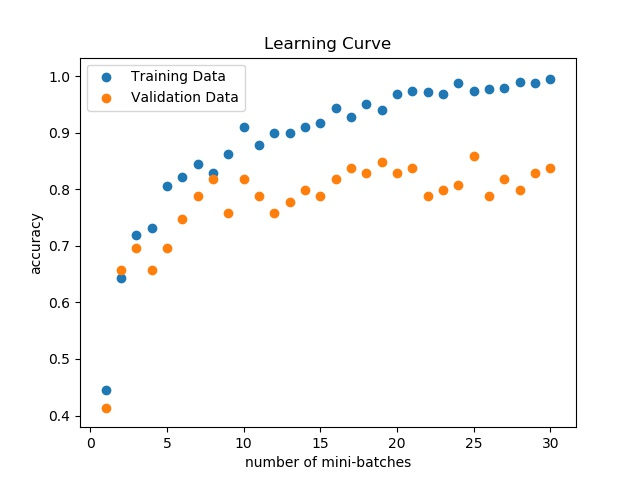
\includegraphics[width=4in]{resources/part8}
         \caption{Learning Curve: the osciallations are due to changing the training set
                  using mini-batches. There are six mini-batches to an epoch.}
       \end{figure}

   Because of the large number of hyperparameters (learning rate, number of epochs, size of the
   training/validation sets, number of neurons in the hidden layer, etc.), it was difficult to
   optimize the network.
   Rather than iteratively fully exploring a subspace of possible hyperparameters (which would grow
   extremely quickly even for few choices for each parameter), the function \texttt{optimize\_params()}
   was used to sample several options, and was run several times with different divisions into
   training/validation/testing sets (changed by setting the seed in \texttt{format\_data()} to 0, 1, 2, and 3).
   The validation results for each set of parameters were then approximately averaged, and that result
   led to a choice of trial 2 (as defined in the \texttt{optimize\_params()} function), i.e. the parameters
   given above. Small changes around these values (particularly increasing the number of epochs)
   had small effects on the results.

   These parameters give a final training accuracy of 99.5\%, validation accuracy of 83.8\%, and
   testing accuracy of 81.7\% (when the data seed is set to 2). While the validation set did have an effect on training through the
   choice of hyper-parameters, this is mitigated by the cross-validation; taking it to be part of
   the testing set gives an accuracy of 82.8\%.
   Averaging the testing accuracy (again including the validation set) over the cross-validation
   samples (i.e. seed of 0,1,2,3) gives an accuracy of 80.5\%.


   \section{Visualizing Weights}
   The following image...

   \section{AlexNet}

\end{document}
